
\chapter{说明}

这册课本是在中小学通用教材物理编写组编的《全日制十年制学校初中课本( 试用本) 物理第二册》的基础上修改而成的。
修改中吸收了几年来各地试用中的一些好经验。许多省市的教师对本书的征求意见稿提了有益的意见和建议。
河北、北京、天津、上海、辽宁、山东、浙江等省市的教研室和教育学院在本书编写过程中给予了大力的支持。在此谨致谢意。

\newpage

\begin{figure}[H]
    \centering
    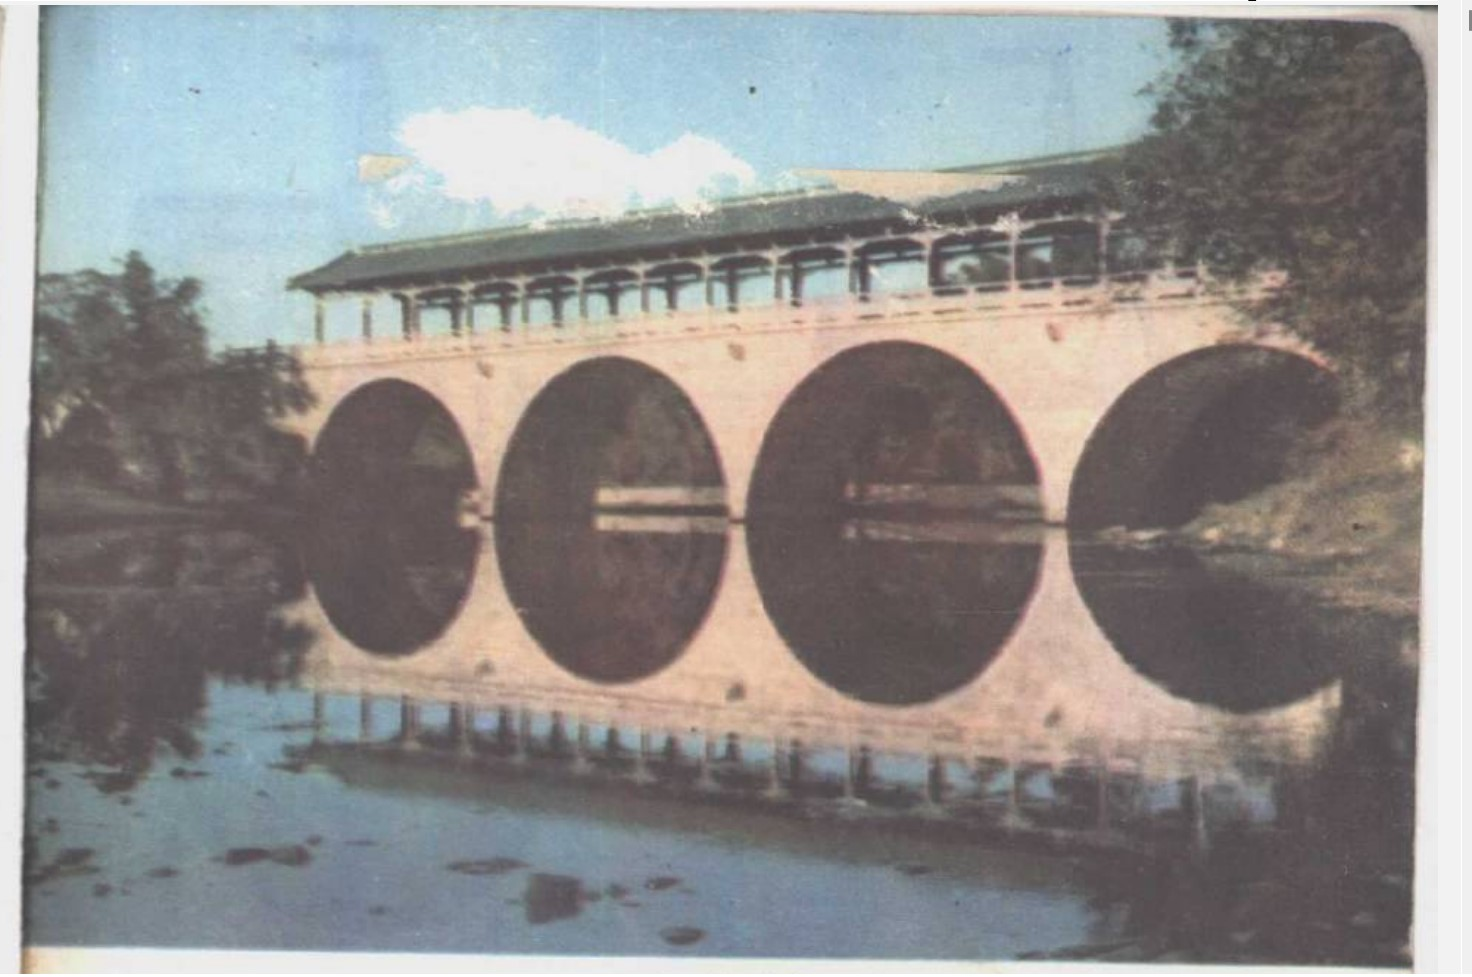
\includegraphics[width=0.95\textwidth]{../pic/czwl2-pic1}
    \caption*{图1 桂林花桥\\(初建于宋代,桥像相连,如月浮江)}\label{fig:pic1}
\end{figure}

\begin{figure}[H]
    \centering
    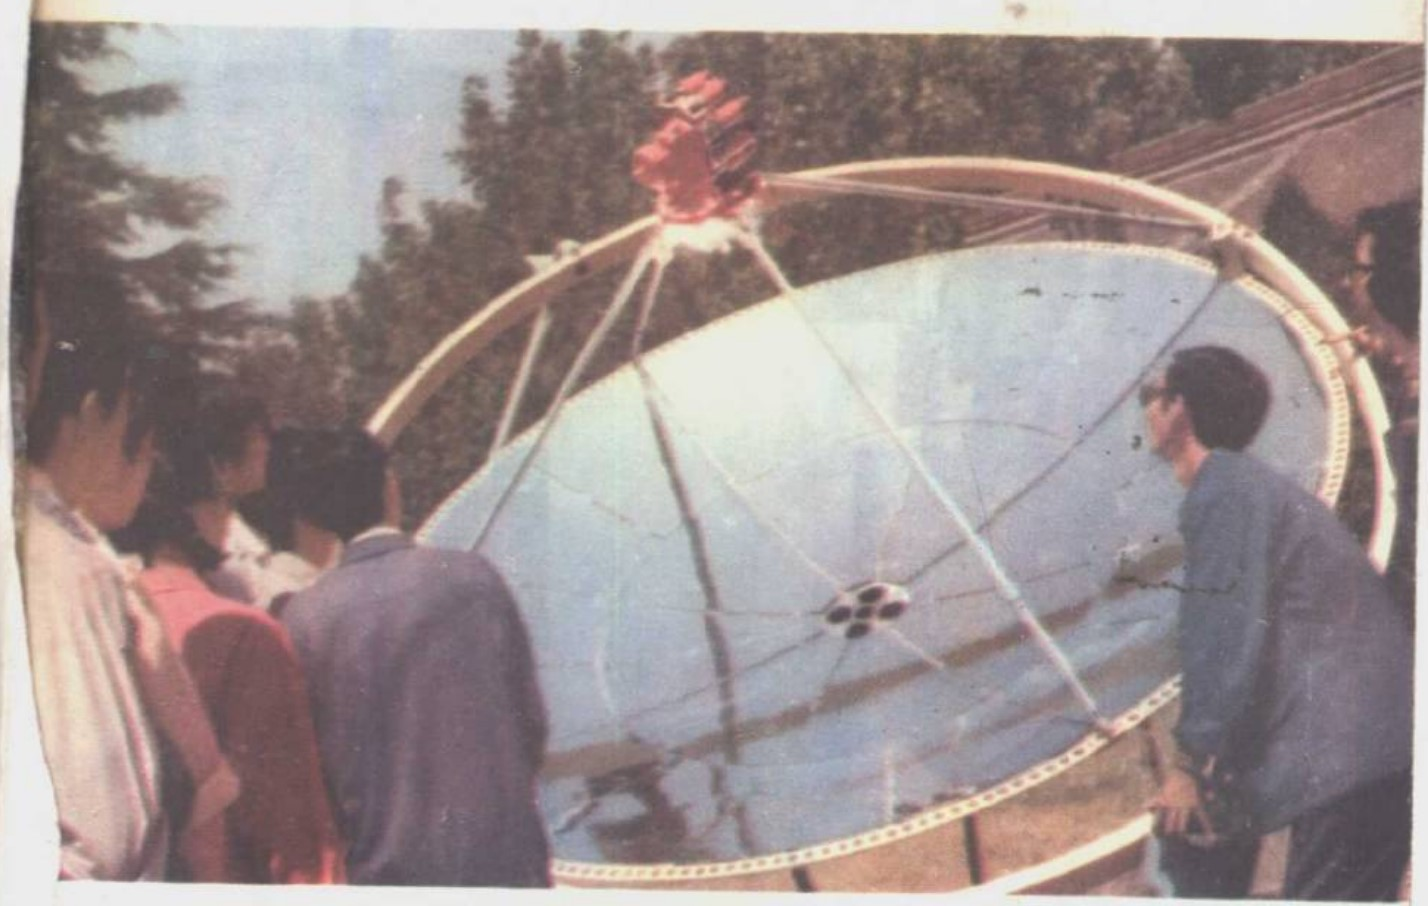
\includegraphics[width=0.95\textwidth]{../pic/czwl2-pic2}
    \caption*{图2 太阳能焊接机}\label{fig:pic2}
\end{figure}

\begin{figure}[H]
    \centering
    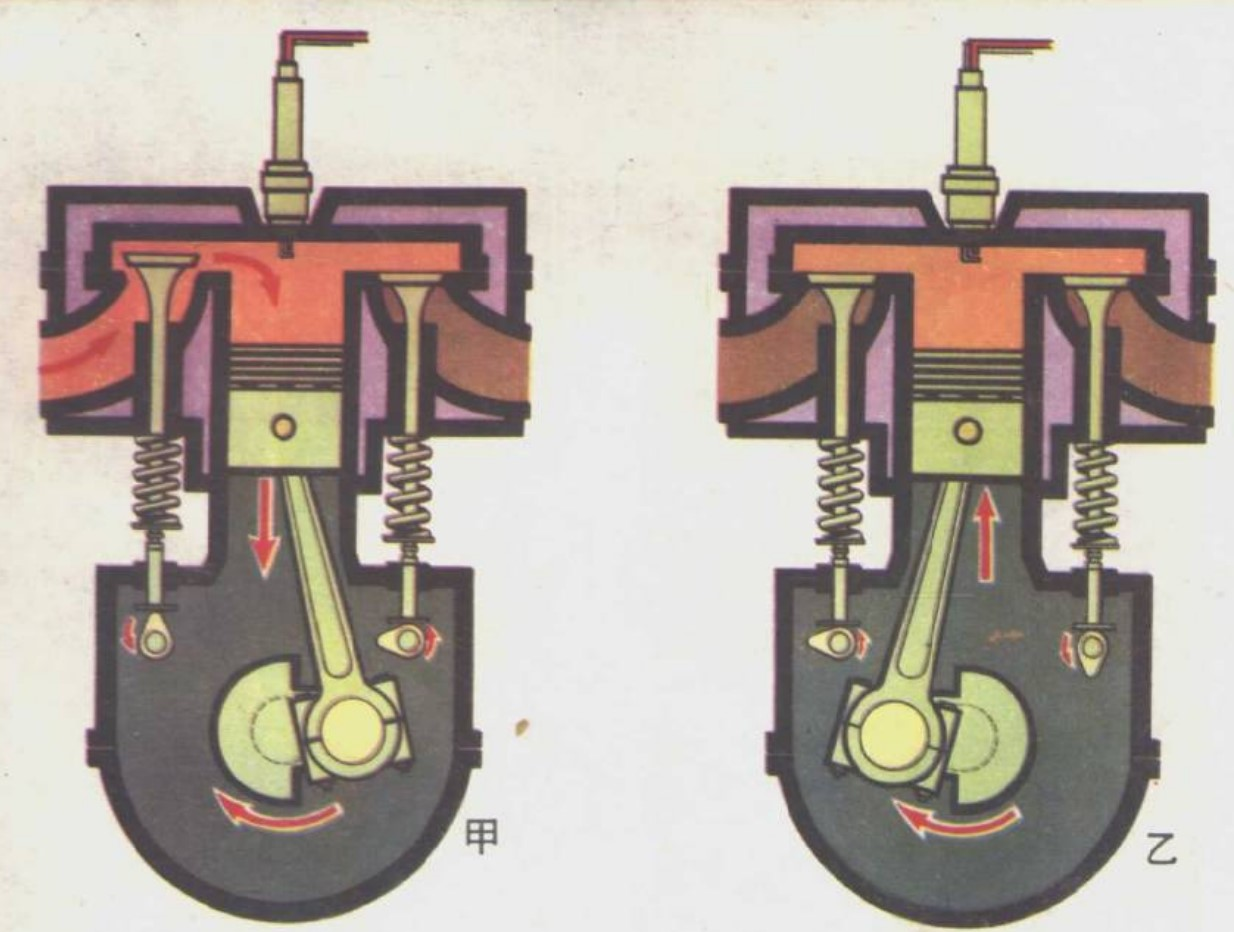
\includegraphics[width=0.95\textwidth]{../pic/czwl2-pic3-a}
    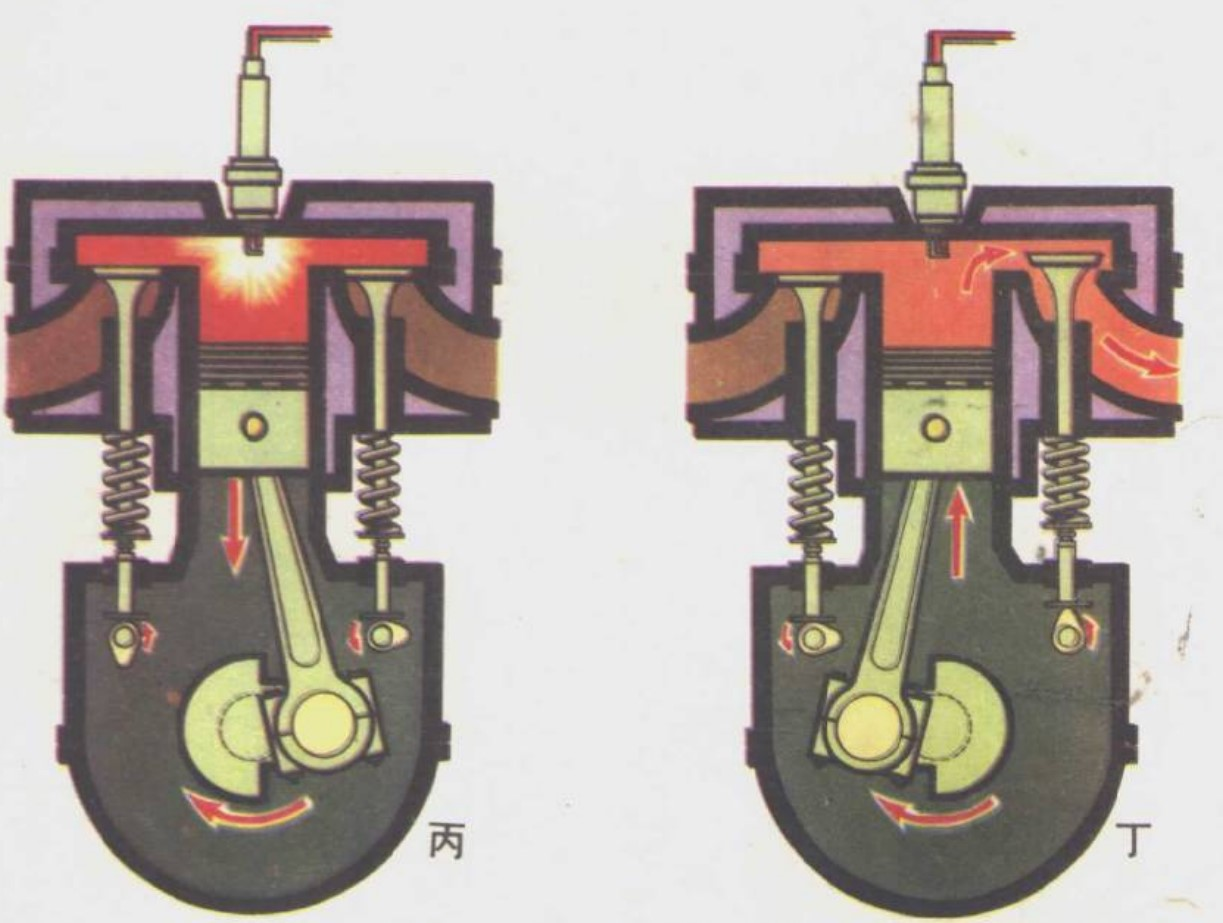
\includegraphics[width=0.95\textwidth]{../pic/czwl2-pic3-b}
    \caption*{图3 汽油机的四个冲程\\(甲 吸气冲程,乙 压缩冲程,丙 做功冲程,丁 排气冲程)}\label{fig:pic3}
\end{figure}
